
\chapter{The 25-Minute Essay}
\section{SAT Worksheet 1D: Warm-up}
\textit{Directions: The below questions are meant to assess what you already know about the SAT Essay. Answer the questions to the best of your ability. }\\

\begin{enumerate}
\item{How is an SAT essay different than the ones that you write for your high school classes?}


\vfill
\item{What is the proper structure of an SAT essay?}


\vfill
\item{How is an SAT essay scored?}


\vfill
\item{What are common errors made on an SAT essay?}

\end{enumerate}
\vfill

\pagebreak
\section{About the SAT Essay}
The SAT essay asks you to present your point of view and support it with examples.  You will usually receive a short excerpt or quote.  Your assignment follows the prompt.  You are asked to support your opinion using reasoning and examples from your reading, studies, experiences, or observations.

\bigskip
You can use examples from…
\begin{itemize}
\item{Literature, describing a character or a theme from a book you understand well and about which you feel comfortable writing.}  
\item{History, describing an event or movement.}
\item{Current events}
\item{Politics}
\end{itemize}

\bigskip
If you are having trouble thinking of more “academic” examples, then you can use...
\begin{itemize}
\item{Literature, describing a character or a theme from a book you understand well and about which you feel comfortable writing.}  
\item{Personal experience - it is okay to use “I”}
\item{Experience of a friend or relative}
\item{Anything that is relevant and will support your point of view!}
\end{itemize}

\bigskip
It is difficult to brainstorm examples on the spot, and students that come prepared with a few strong examples that can be adjusted to answer several different assignments have a major advantage. This is why we will be brainstorming examples later in this class. 

\bigskip
SAT graders are looking for effective writing with a logical and consistent expression of ideas and an insightful, well-supported point of view.

\bigskip
\textit{**Note: it is usually better to “choose a side.”  It is easier to support one point of view than defend both sides of an issue.  It is possible to write a strong essay this way, but it makes your job harder!**}

\pagebreak
\section{Strategies for the SAT Essay}    %The spacing on this was coming out weird on the pdf so because of the different sections, I added a page break before this
\begin{itemize}
\vfill
\item{\textbf{Write neatly.}  The graders need to be able to read your handwriting!}
\vfill

\item{\textbf{Write five paragraphs.}  Try to fill up the space you are given.}


\vfill
\item{\textbf{Take time to understand the prompt.}  An off-topic essay will receive a score of zero.}

\vfill
\item{\textbf{Use strong vocabulary.}  Sprinkle in some of those “ten-dollar” words you've been studying.  However, only use big words if you are sure you are using them correctly.}
\vfill

\item{\textbf{Use transition words.}  Your essay should flow smoothly from one paragraph to the next.  Phrases like ``additionally, consequently, furthermore' enhance logical organization, understandability, and improve the connections between your thoughts.}

\vfill

\item{\textbf{Write topic sentences for each of your “example” paragraphs.}  These will link your examples back to your thesis and show the reader that your essay is on-topic.  }

\vfill
\item{\textbf{Use good time management.} You only have 25 minutes to write the SAT essay.  Manage your time well by spending a few minutes brainstorming and outlining your essay.  Leave a few minutes at the end to proofread your work.}
\end{itemize}

\vfill
\newpage

\section{How an SAT Essay is Scored}
Each essay is independently scored by two readers on a scale from 1 to 6. These readers' scores are combined to produce the 2-12 scale. The essay readers are experienced and trained high school and college teachers.
If the two readers' scores differ by more than one point (a rare situation), a third reader scores the essay.

\begin{center}
\textbf{Scoring Guide}
\end{center}

\bigskip
\underline{Score of 6}

An essay in this category demonstrates clear and consistent mastery, although it may have a few minor errors. A typical essay:

\begin{itemize}
\item{Effectively and insightfully develops a point of view on the issue and demonstrates outstanding critical thinking, using clearly appropriate examples, reasons and other evidence to support its position.}
\item{Is well organized and clearly focused, demonstrating clear coherence and smooth progression of ideas.}
\item{Exhibits skillful use of language, using a varied, accurate and apt vocabulary.}
\item{Demonstrates meaningful variety in sentence structure.}
\item{Is free of most errors in grammar, usage and mechanics.}
\end{itemize}

\vfill
\underline{Score of 5}

An essay in this category demonstrates reasonably consistent mastery, although it has occasional errors or lapses in quality. A typical essay:

\begin{itemize}
\item{Effectively develops a point of view on the issue and demonstrates strong critical thinking, generally using appropriate examples, reasons and other evidence to support its position.}
\item{Is well organized and focused, demonstrating coherence and progression of ideas.}
\item{Exhibits facility in the use of language, using appropriate vocabulary.}
\item{Demonstrates variety in sentence structure.}
\item{Is generally free of most errors in grammar, usage and mechanics.}
\end{itemize}

\vfill
\newpage
\underline{Score of 4}

An essay in this category demonstrates adequate mastery, although it has lapses in quality. A typical essay:
\begin{itemize}
\item{Develops a point of view on the issue and demonstrates competent critical thinking, using adequate examples, reasons and other evidence to support its position}
\item{Is generally organized and focused, demonstrating some coherence and progression of ideas.}
\item{Exhibits adequate but inconsistent facility in the use of language, using generally appropriate vocabulary.}
\item{Demonstrates some variety in sentence structure.}
\item{Has some errors in grammar, usage and mechanics.}
\end{itemize}

\vfill
\underline{Score of 3}

An essay in this category demonstrates developing mastery, and is marked by ONE OR MORE of the following weaknesses:

\begin{itemize}
\item{Develops a point of view on the issue, demonstrating some critical thinking, but may do so inconsistently or use inadequate examples, reasons or other evidence to support its position.}
\item{Is limited in its organization or focus, or may demonstrate some lapses in coherence or progression of ideas.}
\item{Displays developing facility in the use of language, but sometimes uses weak vocabulary or inappropriate word choice.}
\item{Lacks variety or demonstrates problems in sentence structure.}
\item{Contains an accumulation of errors in grammar, usage and mechanics.}
\end{itemize}

\vfill
\underline{Score of 2}

An essay in this category demonstrates little mastery, and is flawed by ONE OR MORE of the following weaknesses:

\begin{itemize}
\item{Develops a point of view on the issue that is vague or seriously limited, and demonstrates weak critical thinking, providing inappropriate or insufficient examples, reasons or other evidence to support its position.}
\item{Is poorly organized and/or focused, or demonstrates serious problems with coherence or progression of ideas.}
\item{Displays very little facility in the use of language, using very limited vocabulary or incorrect word choice.}
\item{Demonstrates frequent problems in sentence structure.}
\item{Contains errors in grammar, usage and mechanics so serious that meaning is somewhat obscured.}
\end{itemize}

\vfill
\underline{Score of 1}

An essay in this category demonstrates very little or no mastery, and is severely flawed by ONE OR MORE of the following weaknesses:

\begin{itemize}
\item{Develops no viable point of view on the issue, or provides little or no evidence to support its position.}
\item{Is disorganized or unfocused, resulting in a disjointed or incoherent essay.}
\item{Displays fundamental errors in vocabulary.}
\item{Demonstrates severe flaws in sentence structure.}
\item{Contains pervasive errors in grammar, usage or mechanics that persistently interfere with meaning.}
\end{itemize}

\bigskip
\underline{Score of 0}

Essays not written on the essay assignment will receive a score of zero.

\vfill
\newpage
\section[Getting A Perfect Score]{Secrets to Getting a Perfect Score on an SAT Essay}
An essay with the following elements done completely will have a good chance of getting a perfect score:

\bigskip
\begin{itemize}
\vfill\item Strong and interesting introduction
\vfill\item Clear thesis (presented at the end of the introductory paragraph)
\vfill\item Well worded and clear topic sentence for paragraph 1
\vfill\item Well explained example in the body paragraph 1
\vfill\item Good transition between body paragraphs 1 and 2
\vfill\item Well worded and clear topic sentence for paragraph 2
\vfill\item Well explained example in the body paragraph 2
\vfill\item Good transition between body paragraphs 2 and 3
\vfill\item Well worded and clear topic sentence for paragraph 3
\vfill\item Well explained example in the body paragraph 3
\vfill\item Good transition between paragraphs 3 and 4
\vfill\item Conclusion that recaps the thesis
\vfill\item Conclusion extends the essay beyond recapping the thesis
\vfill\item Correct grammar
\vfill\item Sophisticated vocabulary
\vfill\item Varied sentence structure and appropriate syntax
\end{itemize}
\vfill

\newpage
Graphic Organizers such as the ones below can help you to organize your essay:

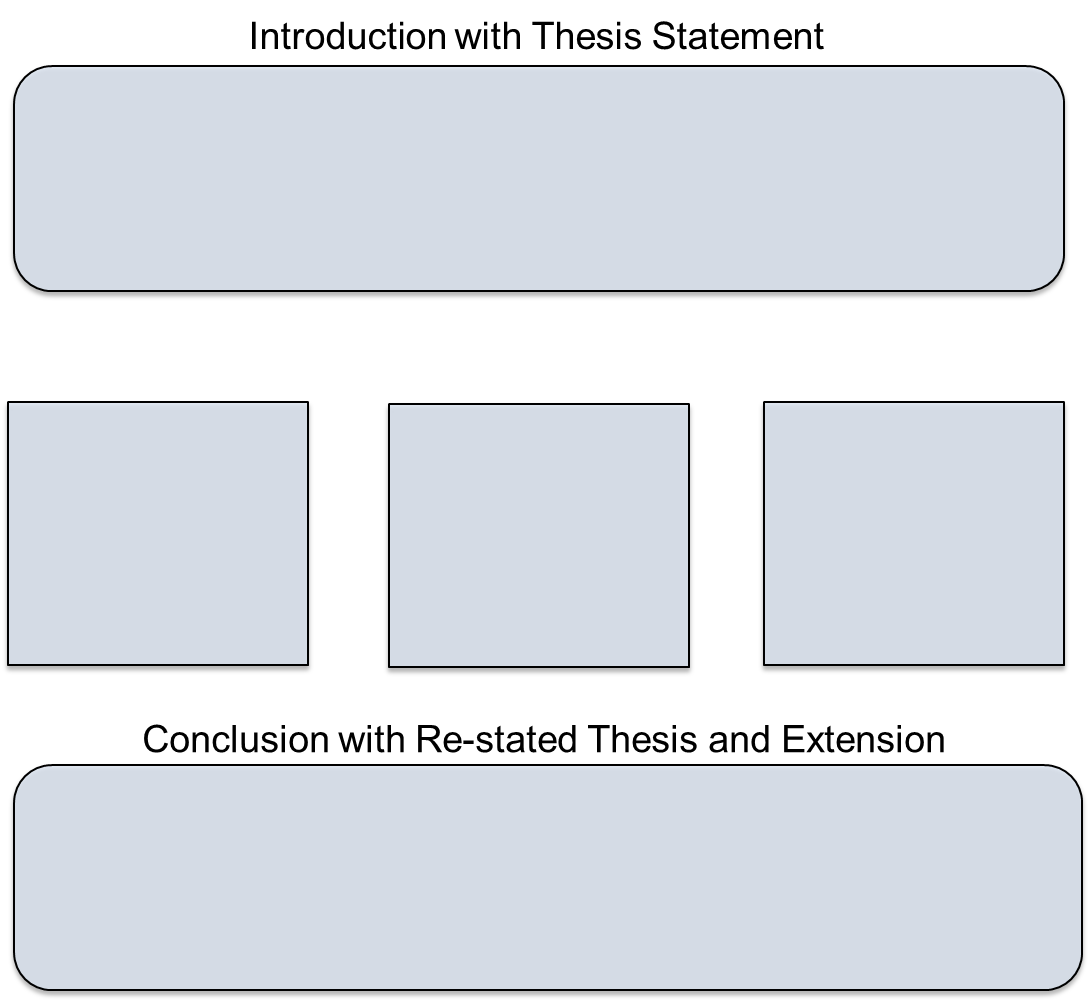
\includegraphics[width=\textwidth]{Organizer}

\section[Scoring]{SAT Worksheet 2D: Practice Scoring an SAT Essay}
\textit{Directions: Read the following assignment and essay response written in 25 minutes. Then, answer the questions that follow.}

\bigskip
Assignment: Do changes in our lives necessarily make them better? Plan and write an essay in which you develop your point of view on this issue.  Support your position with reasoning and examples taken from your reading, studies, experience, or observations.

\bigskip
\indent In the 18th century, many women were burdened with the difficult task of washing clothes by hand. While some women may have taken pride in this task, the invention of the washing machine enabled these women to spend more time with other tasks and move beyond household chores. While this is an example of how changes that make our lives easier can also make them better, it is not always true that the changes that make our lives easier do not always improve them.\\

\indent The research surrounding household appliances-including that presented in the book, “The World is Fat”-demonstrates that while housekeeping luxuries have made our lives easier have not necessarily improved them. For example, an advantage of appliances such as washers and dryers have made our lives easier because they have decreased the average time that an American adult spends on household chores per day. However, this progress is a double-edged sword because in decreasing the amount of time spent on tasks such as cleaning floors and washing dishes, these devices have also decreased the amount of calories that Americans burn while completing these tasks. “The World is Fat” author bemoans this as a major contributing factor to obesity crisis in America. Since calories can be correlated with amount of time on chores, it is clear that household appliances have come with a Catch-22. \\

\indent In addition to household appliances, another aspect of modern technology, social media, have made our lives easier without becoming purely better. While social media has made it more convenient to communicate with our friends, it has also been the source of many problems. For example, an issue prevalent in the lives of many American teenagers is cyber-bullying. Social media sites such as Facebook have enabled students to tease or harass other students. This situation is detrimental to the mental health of both the bully and the bullied students. As a result, in making communication between people easier, social media has had unintended consequences, such as cyberbulling, that do not necessarily improve our lives. \\

\indent In analyzing the effects of household appliances and social media, it is clear that easy does not always facilitate improved well being. This leads me to believe that when inventors and other innovators are considering bringing a product to market, they should consider the question of “will this thing help others?” in addition to the consideration of whether or not it will make other's lives easier. Consideration of both of these questions could help to safeguard American society.  

\bigskip
\begin{enumerate}
\item{\textbf{What are things that the essay does well?}}
\vfill
\item{\textbf{What are things that this essay could improve upon?}}
\vfill
\item{\textbf{If you were an SAT scorer, what score (0-6) would you give this essay?}}
\vfill
\end{enumerate}

\newpage
\section[Brainstorming Ideas]{SAT Worksheet 3D: Brainstorming Examples}
\bigskip
\textit{Directions: Below are examples of categories that you can use in the body paragraphs of your SAT essays. Brainstorm as many examples as you can for each category and write an example of the types of essays it could be used for. For example, the “Harry Potter” series could be used in an essay about whether it is better to work alone or with a group.}

\begin{spacing}{2}
\textbf{Literature}
\begin{enumerate}
\item For example: ``The Harry Potter series'' could be used in an essay about individualism versus teamwork
\item
\item
\item
\end{enumerate}

\vfill
\textbf{History}
\begin{enumerate}
\item
\item
\item
\item
\end{enumerate}

\vfill
\textbf{Current Events}
\begin{enumerate}
\item
\item
\item
\item
\end{enumerate}
\end{spacing}

\newpage
\begin{spacing}{2}
\textbf{Politics}

\begin{enumerate}
\item
\item
\item
\item
\end{enumerate}

\vfill
\textbf{Personal Experiences}

\begin{enumerate}
\item
\item
\item
\item
\end{enumerate}

\vfill
\textbf{Experiences of Someone else}

\begin{enumerate}
\item
\item
\item
\item
\end{enumerate}
\end{spacing}
\vfill\vfill
\newpage

\section{Transition Words}
Effective use of transitional words and phrases enhances the flow and consistency of your essay. 

\bigskip
Transitions help papers read more smoothly and strengthen connections between ideas.  Just as topic sentences help link your examples back to your thesis statement, transitions also act as the “glue” that binds your ideas together and keeps your entire essay focused and on-topic.

\bigskip
\textit{Avoid weak topic sentences like, ``My first example is"...``My second example is..."}

\bigskip
\underline{Transition words and phrases of:}

\bigskip
\textbf{Addition:}\\
also, again, as well as, besides, coupled with, furthermore, in addition, likewise, moreover, similarly

\bigskip
\textit{In The Great Gatsby, the main character Jay Gatsby demonstrates an inability to move on from his past.  Ethan Frome, similarly, is a literary character who is haunted by his past and cannot succeed in his present.}

\bigskip
\textbf{Consequence:}\\
accordingly, as a result, consequently, for this reason, for this purpose, hence, otherwise, so then, subsequently, therefore, thus, thereupon, wherefore

\bigskip
\textit{He never called in his absence from work, and consequently got fired the next day.}

\bigskip
\textbf{Contrast and Comparison:}\\
contrast, by the same token, conversely, instead, likewise, on one hand, on the other hand, on the contrary, rather, similarly, yet, but, however, still, nevertheless, in contrast

\bigskip
\textit{I can't wait to get a puppy; however, I understand dog ownership is a big responsibility.}

\bigskip
\textbf{Diversion:}
by the way, incidentally

\bigskip
\textit{Susie got in trouble for skipping class on Thursday.  Incidentally, I skipped class that day too.}

\bigskip
\textbf{Emphasis:}\\
above all, chiefly, with attention to, especially, particularly, singularly

\bigskip
\textit{I focused particularly on studying for my Spanish test, because learning foreign languages is my biggest challenge. }

\bigskip
\textbf{Exception:}\\
aside from, barring, besides, except, excepting, excluding, exclusive of, other than, outside of, save, apart from

\bigskip
\textit{Besides Alicia, who else plays an instrument in a band?}

\bigskip
\textbf{Exemplifying:}\\
chiefly, especially, for instance, in particular, markedly, namely, particularly, including, specifically, such as

\bigskip
\textit{Granada, Spain is famous for its Moorish architecture, especially its beautiful palace, the Alhambra.}

\bigskip
\textbf{Generalizing:}\\
as a rule, as usual, for the most part, generally, generally speaking, ordinarily, usually

\bigskip
\textit{Generally speaking, third graders choose recess over math class.}

\bigskip
\textbf{Illustration:}\\
for example, for instance, for one thing, as an illustration, illustrated with, as an example, in this case


\bigskip
\textit{Resistance to totalitarian rule is a common theme throughout young adult literature.  Katniss Everdeen, for example, becomes a symbol for the resistance against the brutally oppressive Capitol in Suzanne Collins' The Hunger Games.}

\bigskip
\textbf{Similarity:}\\
comparatively, coupled with, correspondingly, identically, likewise, similar, moreover, together with

\bigskip
\textit{As the deadline drew closer, her stress levels correspondingly grew higher.}

\bigskip
\textbf{Restatement:}\\
in essence, in other words, namely, that is, that is to say, in short, in brief, to put it differently

\bigskip
\textit{For all his posturing, he is actually, in essence, a down-to-earth and humble person.}

\bigskip
\textbf{Sequence:}\\
at first, first of all, to begin with, in the first place, at the same time, for now, for the time being, the next step, in time, in turn, later on, meanwhile, next, then, soon, the meantime, later, while, earlier, simultaneously, afterward, in conclusion, with this in mind

\bigskip
\textit{It is dangerous and illegal to simultaneously text and drive.}

\bigskip
\textbf{Summarizing:}\\
after all, all in all, all things considered, briefly, by and large, in any case, in any event, in brief, in conclusion, on the whole, in short, in summary, in the final analysis, in the long run, on balance, to sum up, to summarize, finally

\bigskip
\textit{We lost our final baseball game, but all in all we had a successful season.}

\pagebreak

\section[Essay Prompts]{SAT Worksheet 4D: SAT Essay Prompts}

\textit{Directions: Think carefully about the issue presented in the following excerpt and the assignment below.}

\begin{enumerate}
\item{\textbf{Prompt 1}}

\textit{``It is good to have an end to journey toward; but it is the journey that matters, in the end."}  \\ 
-Ernest Hemingway.

\bigskip
\textbf{Assignment:} Is the destination as significant as the journey to get there?  Plan and write an essay in which you develop your point of view on this issue.  Support your position with reasoning and examples taken from your reading, studies, experience, or observations.

\item{\textbf{Prompt 2}}\\
\textit{``Technological progress has merely provided us with more efficient means for going backwards."}\\
-Aldous Huxley

\bigskip
\textbf{Assignment:} Does technological advancement cause humans to regress or advance?  Plan and write an essay in which you develop your point of view on this issue.  Support your position with reasoning and examples taken from your reading, studies, experience, or observations.

\item{\textbf{Prompt 3}}\\
\textit{``Ours is a world of nuclear giants and ethical infants. We know more about war than we know about peace, more about killing than we know about living."}\\
-Omar Nelson Bradley

\bigskip
\textbf{Assignment:}Are people more prone to acts of aggression than acts of peace?  Plan and write an essay in which you develop your point of view on this issue.  Support your position with reasoning and examples taken from your reading, studies, experience, or observations.
\end{enumerate}
